\documentclass[12pt]{amsart}
\usepackage{amsmath}
\usepackage{amsfonts}
\usepackage{tikz}

\addtolength{\oddsidemargin}{-0.5in}
\addtolength{\evensidemargin}{-0.5in}
\addtolength{\textwidth}{1.0in}
\addtolength{\topmargin}{-1.0in}
\addtolength{\textheight}{1.0in}

\begin{document}

\centerline{\bf MATH 738}
\centerline{\bf HW 1} 
\centerline{\bf Due 9/15}

\vspace{2em}

% -Isomorphisms induce natural isomorphism of h_X
% -Check that F^{-1} on morphism is also a functor. 
% -Units/counits <=> adjunction
% -Complete the proof of Tensor-Hom adjunction, check natural transformation 
% -Inverse of natural isomorphism is an natural transformation

\begin{enumerate}
    
    \item Let $\phi : X \to X^\prime$ be an isomorphism in a category $\mathcal C$. Show that 
    \begin{align*}
        \operatorname{Hom}(X^\prime,Y) & \to \operatorname{Hom}(X,Y) \\
        \psi & \mapsto \psi \circ \phi
    \end{align*}
    is a bijection. Show that it induces an isomorphism $h_X \cong h_{X^\prime}$. 

    \item In the proof that a fully-faithful and essential surjective functor is an equivalence, we 
    constructed what we claimed was the inverse. Show that it is well-defined and indeed the inverse functor. 

    \item Prove that $F \vdash G$ if and only if there exists $\eta : \operatorname{Id} \to GF$ and $\eta 
    : FG \to \operatorname{Id}$ satsifying 
    \begin{center}
    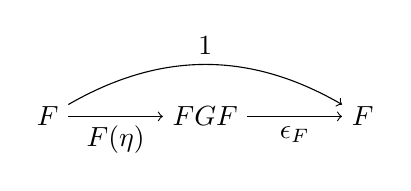
\begin{tikzpicture}
        \node at (0,0) (F1) {$F$};
        \node at (2,0) (FGF) {$FGF$};
        \node at (4,0) (F2) {$F$};
        \draw[->] (F1) -- node[below] {$F(\eta)$} (FGF);
        \draw[->] (FGF) -- node[below] {$\epsilon_F$} (F2);
        \draw[->] (F1) to [out=30,in=150] node[above] {$1$} (F2); 
    \end{tikzpicture}
    \end{center}
    and 
    \begin{center}
    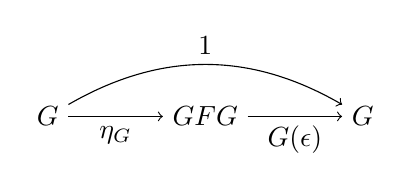
\begin{tikzpicture}
        \node at (0,0) (G1) {$G$};
        \node at (2,0) (GFG) {$GFG$};
        \node at (4,0) (G2) {$G$};
        \draw[->] (G1) -- node[below] {$\eta_G$} (GFG);
        \draw[->] (GFG) -- node[below] {$G(\epsilon)$} (G2);
        \draw[->] (G1) to [out=30,in=150] node[above] {$1$} (G2);
    \end{tikzpicture}
    \end{center}

    \item Complete the proof of tensor-hom adjunction. Show that the claimed inverse natural transformation is 
    well-defined and indeed the inverse. 

\end{enumerate}

\end{document}